%https://tex.stackexchange.com/questions/164991/pgfplots-how-to-fill-bounded-area-under-a-curve-using-addplot-and-fill

%https://tex.stackexchange.com/questions/140312/tikz-shading-region-bounded-by-several-curves
%tikz para graficar areas

%http://latexcolor.com/

%https://www.tablesgenerator.com/
\PassOptionsToPackage{force}{filehook}

\documentclass{beamer}


\usepackage[utf8]{inputenc}
\usepackage{amsmath}
\usepackage{amssymb}% http://ctan.org/pkg/amssymb
\usepackage{amsfonts}
\usepackage{pifont}% http://ctan.org/pkg/pifont
%https://tex.stackexchange.com/questions/42619/x-mark-to-match-checkmark
\newcommand{\cmark}{\ding{51}}
\newcommand{\xmark}{\ding{55}}
%\usepackage{amsfonts}
\usepackage{graphicx} 
\usepackage{subcaption}
\usepackage{hyperref}
\usepackage{cancel}
\usepackage{wrapfig}
\usepackage{enumitem}
\usepackage{comment}
\hypersetup{
	colorlinks=true,
	linkcolor=blue,
	filecolor=magenta,      
	urlcolor=cyan,
}
\newtheorem*{proposicion}{Proposici\'on}
\newtheorem*{teorema}{Teorema}
\renewcommand*{\proofname}{Demostraci\'on}
\newtheorem*{ejercicio}{Ejercicio}
\usepackage{pgf,tikz}
\usetikzlibrary{positioning}
\usetikzlibrary{arrows,patterns}
\usetikzlibrary{arrows.meta}
\usepackage[spanish, activeacute]{babel} %Definir idioma español
\usepackage[utf8]{inputenc} %Codificacion utf-8
\usepackage{multirow}

%   Esconder las soluciones
\newif\ifhideproofs
\hideproofstrue %uncomment to hide proofs

\ifhideproofs
\usepackage{environ}
\NewEnviron{hide}{}
\let\solucion\hide
\let\endsolucion\endhide
\fi

\usepackage{color}
\usepackage{mathpazo}
\usepackage{hyperref}
\usepackage{multimedia}
\usepackage{graphicx}
\usepackage{textcomp}
\usepackage[spanish, activeacute]{babel} 
\usepackage{graphicx} 
\usepackage{booktabs}
\usepackage{cite}
\usepackage{hyperref}
\usepackage{multicol}
\usepackage{multirow,array}

\usepackage{mathrsfs}
\decimalpoint
%\usepackage{amssymb}

\usepackage{tabularx}
    \newcolumntype{L}{>{\raggedright\arraybackslash}X}
        %\newcolumntype{b}{>{\hsize=1.5\hsize}X}
    %\newcolumntype{s}{>{\hsize=.9\hsize}X}

\usepackage{amsthm}
\newtheorem{thm}{Teorema}
\newtheorem{lem}[thm]{Lema}
\newtheorem{axiom}[thm]{Axioma}
\newtheorem{prop}[thm]{Proposici\'on}
\newtheorem{coro}[thm]{Corolario}
\theoremstyle{definition}
\newtheorem{defn}{Definici\'on}
\DeclareGraphicsExtensions{.pdf,.jpeg,.png,.eps}
\usetheme{CambridgeUS}
\setbeamertemplate{navigation symbols}{}

%Paréntisis y otros
\newcommand{\cmc}{\overset{m.c.}{\rightarrow}}
\newcommand{\p}[1]{\left(#1\right)}
\newcommand{\cor}[1]{\left[#1\right]}
\newcommand{\lla}[1]{\left\{#1\right\}}
\newcommand{\eps}{\varepsilon}
\newcommand{\lol}{\mathcal{L}}
\newcommand{\RR}{\mathbb{R}}
\newcommand{\QQ}{\mathbb{Q}}
\newcommand{\NN}{\mathbb{N}}
\newcommand{\paren}[1]{\left(#1\right)}
\newcommand{\corc}[1]{\left[#1\right]}
\newcommand{\llav}[1]{\left\lbrace#1\right\rbrace}
\newcommand{\partt}[1]{\left(\text{#1}\right)}
\newcommand{\corctt}[1]{\left[\text{#1}\right]}
\newcommand{\llavtt}[1]{\left\lbrace\text{#1}\right\rbrace}
\makeatletter
\def\munderbar#1{\underline{\sbox\tw@{$#1$}\dp\tw@\z@\box\tw@}}
\makeatother

%\usepackage[scr=rsfs,cal=boondox]{mathalfa}
\usepackage[scr=esstix,cal=boondox]{mathalfa}

% \usepackage{mdframed}
% \newmdtheoremenv{solucion}{Soluci\'on}

% Enmarcar las soluciones
% \newenvironment{solu}
% {%
% \begin{framed}
%   \begin{solucion}
%   }%
%     {%     
%   \end{solucion}
% \end{framed}
% }

%   Esconder las soluciones
\newif\ifhideproofs
%\hideproofstrue %uncomment to hide proofs

\ifhideproofs
\usepackage{environ}
\NewEnviron{hide}{}
\let\solucion\hide
\let\endsolucion\endhide
\fi



%Graficos y cosas
\usepackage{amssymb}
\usepackage{tikz}
\usepackage{pgfplots}
\usepackage{mathtools}
\usepackage{xcolor}
%\pgfplotsset{compat=1.9}
\usepgfplotslibrary{fillbetween,decorations.softclip}
\pgfplotsset{compat = newest}
\usepackage{pst-func}
\usepackage{pstricks}
\usepackage{pst-plot}

% Comando para usar multiples footnotes en un align environment

\makeatletter
\newcommand{\AlignFootnote}[1]{%
    \ifmeasuring@
    \else
        \footnote{#1}%
    \fi
}
\makeatother

%https://tex.stackexchange.com/questions/82782/footnote-in-align-environment


\DeclareGraphicsExtensions{.pdf,.jpeg,.png,.eps}
\usepackage{tikz}
%\usepackage{tikz-cd}
\usetikzlibrary{decorations}
%\usetikzlibrary{snakes}
\usetikzlibrary{cd}

\useoutertheme{split}
\useinnertheme{rounded}


%\beamertemplatenavigationsymbolsempty  %removes navigation bar
\definecolor{rosee}{rgb}{0.7,0.05,0.25}
\definecolor{pacificorange}{cmyk}{0,.6,1,0} %approved Pacific colors 2010
\definecolor{pacificgray}{cmyk}{0,.15,.35,.60}
\definecolor{pacificlgray}{cmyk}{0,0,.2,.4}
\definecolor{pacificcream}{cmyk}{.05,.05,.15,0}
\definecolor{deepyellow}{cmyk}{0,.17,.80,0}
\definecolor{lightblue}{cmyk}{.49,.01,0,0}
\definecolor{lightbrown}{cmyk}{.09,.15,.34,0}
\definecolor{deepviolet}{cmyk}{.79,1,0,.15}
\definecolor{deeporange}{cmyk}{0,.59,1,18}
\definecolor{dustyred}{cmyk}{0,.7,.45,.4}
\definecolor{grassgreen}{RGB}{92,135,39}
\definecolor{pacificblue}{RGB}{59,110,143}
\definecolor{pacificgreen}{cmyk}{.15,0,.45,.30}
\definecolor{deepblue}{cmyk}{1,.57,0,2}
\definecolor{turquoise}{cmyk}{.43,0,.24,0}
\definecolor{gren}{rgb}{0.2,0.8,0.5}
\definecolor{orang}{rgb}{1,0.64,0}
\definecolor{amethyst}{rgb}{0.6, 0.4, 0.8}
\definecolor{dodgerblue}{rgb}{0.12, 0.56, 1.0}
\definecolor{fandango}{rgb}{0.71, 0.2, 0.54}
\definecolor{forestgreen(traditional)}{rgb}{0.0, 0.27, 0.13}
\definecolor{iris}{rgb}{0.35, 0.31, 0.81}
\definecolor{jazzberryjam}{rgb}{0.65, 0.04, 0.37}
\definecolor{mediumjunglegreen}{rgb}{0.11, 0.21, 0.18}
\definecolor{mediumpersianblue}{rgb}{0.0, 0.4, 0.65}
\definecolor{midnightgreen}{rgb}{0.0, 0.29, 0.33}
\definecolor{orangee}{rgb}{1.0, 0.5, 0.0}

% There are many different themes available for Beamer. A comprehensive
% list with examples is given here:
% http://deic.uab.es/~iblanes/beamer_gallery/index_by_theme.html
% You can uncomment the themes below if you would like to use a different
% one:
%\usetheme{AnnArbor} %boca
%\usetheme{Antibes} %azul y gris
%\usetheme{Bergen} %barra who where
%\usetheme{Berkeley} %bordes
%usetheme{Berlin} %blanco y azul
%\usetheme{Boadilla}
%\usetheme{boxes}
\usetheme{CambridgeUS}
%\usetheme{Copenhagen}
%\usetheme{Darmstadt}
%\usetheme{default}
%\usetheme{Frankfurt}
%\usetheme{Goettingen}
%\usetheme{Hannover}
%\usetheme{Luebeck}
%\usetheme{Malmoe}
%\usetheme{Marburg}
%\usetheme{Montpellier}
%\usetheme{PaloAlto}
%\usetheme{Pittsburgh}
%\usetheme{Rochester}
%\usetheme{Singapore}
%\usetheme{Szeged}
%\usetheme{Warsaw}

%\usecolortheme{beaver}
%\usecolortheme{whale}
%\usecolortheme{orchid}
%\usecolortheme{wolverine}
%\usecolortheme[named=pacificblue]{structure} %replaces the blue of Copenhagen with Pacific orange

\definecolor{myNewColorA}{rgb}{0,0,100}
\definecolor{myNewColorB}{rgb}{0,100,100}
\definecolor{myNewColorC}{rgb}{0,200,100}
\definecolor{myNewColorD}{rgb}{0,100,200}

%\setbeamercolor*{palette primary}{bg=myNewColorA, fg = black}
%\setbeamercolor*{palette secondary}{bg=myNewColorB, fg = black}
%\setbeamercolor*{palette tertiary}{bg=myNewColorC, fg = black}
%\setbeamercolor*{palette quaternary}{bg=myNewColorD, fg = black}

\setbeamercolor*{palette primary}{bg=rosee, fg = white}
\setbeamercolor*{palette secondary}{bg=gren, fg = white}
\setbeamercolor*{palette tertiary}{bg=-red!75!, fg = white}
\setbeamercolor*{palette quaternary}{bg=-red!75!, fg = white}



%\expandafter\def\expandafter\insertshorttitle\expandafter{%
 % \insertshorttitle\hfill%
  %\insertframenumber\,/\,\inserttotalframenumber}

%\mode
%<all>

%Para agrandar el espacio entre renglones de las tablas
%https://tex.stackexchange.com/questions/26690/how-to-add-extra-spaces-between-rows-in-tabular-environment
\renewcommand{\arraystretch}{1.5}

\usepackage{color, xcolor}
\definecolor{codegreen}{rgb}{0,0.6,0}
\definecolor{codegray}{rgb}{0.5,0.5,0.5}
\definecolor{codepurple}{rgb}{0.58,0,0.82}
\definecolor{backcolour}{rgb}{0.95,0.95,0.92}

\usepackage{listings}
\lstdefinestyle{mystyle}{
  backgroundcolor=\color{backcolour},   
  commentstyle=\color{codegreen},
  language = R,
  % commentchar=\#,
  keywordstyle=\color{magenta},
  numberstyle=\tiny\color{codegray},
  stringstyle=\color{codepurple},
  basicstyle=\ttfamily\footnotesize,
  breakatwhitespace=false,         
  breaklines=false,                 
  captionpos=b,                    
  frame=single,
  keepspaces=false,
  % numbers=left,                    
  % numbersep=pt,                  
  % columns=flexible,
  stepnumber=1,
  resetmargins=true,
  showspaces=false,                
  showstringspaces=false,
  showtabs=false,                  
  tabsize=1
}
\lstset{style=mystyle}
  



\def\mydate{\leavevmode\hbox{\twodigits\day/\twodigits\month/\the\year}}
\def\twodigits#1{\ifnum#1<10 0\fi\the#1}

\usepackage[final]{pdfpages}

\newcommand{\shrug}[1][]{%
\begin{tikzpicture}[baseline,x=0.8\ht\strutbox,y=0.8\ht\strutbox,line width=0.125ex,#1]
\def\arm{(-2.5,0.95) to (-2,0.95) (-1.9,1) to (-1.5,0) (-1.35,0) to (-0.8,0)};
\draw \arm;
\draw[xscale=-1] \arm;
\def\headpart{(0.6,0) arc[start angle=-40, end angle=40,x radius=0.6,y radius=0.8]};
\draw \headpart;
\draw[xscale=-1] \headpart;
\def\eye{(-0.075,0.15) .. controls (0.02,0) .. (0.075,-0.15)};
\draw[shift={(-0.3,0.8)}] \eye;
\draw[shift={(0,0.85)}] \eye;
% draw mouth
\draw (-0.1,0.2) to [out=15,in=-100] (0.4,0.95); 
\end{tikzpicture}}

% PARA AGREGAR IMAGEN EN EL FONDO DE LAS SLIDES
\usebackgroundtemplate%
%{%
 %
\includegraphics[width=\paperwidth,height=\pape%rheight]{slides1/fondo.png}%  
%}


\title{\color{black}{Análisis Estadístico}}
\subtitle{\color{rosee}Introducción\\ \color{rosee}\mydate}
\author[Introducción]{}%{Lara Sánchez Peña\footnote{Basado en las notas de Ezequiel Smucler}}
\institute[]{UTDT}
\medskip
\date[UTDT 2021]{}

\begin{document}
\begin{frame}
  \titlepage
\end{frame}

\begin{frame}{\color{rosee}Objetivos generales del curso${}^*$}
\begin{enumerate}
    \item Presentación
    \item Programa
    \item Expectativa del curso y recomendaciones \href{https://www.youtube.com/watch?v=eorGIZ0Y8RY&ab_channel=Nerdforge}{1h - 10h -100h}
\end{enumerate}

    \begin{itemize}
    \item Introducción a los problemas de inferencia (cuando y para qué hacer inferencia estadística).\medskip
        \item Introducción de las herramientas (métodos) fundamentales de inferencia: \medskip
            \begin{itemize}
        \item Estimación puntual. \medskip 
        \item Estimación por intervalos.\medskip
        \item Testeo de hipótesis.\medskip
            \end{itemize}
        \item Caracterizar ciertas propiedades de los métodos de inferencia.\medskip
                    \begin{itemize}
        \item Consistencia, nociones de optimalidad, propiedades asintóticas...\medskip
            \end{itemize}
    \end{itemize}
\end{frame}

\begin{frame}{\color{rosee}Objetivos de la clase${}^*$}
    \begin{itemize}
    \item ¿Qué es la \textbf{inferencia} estadística/ el análisis estadístico?
        \item ¿Para qué usamos la inferencia estadística?
        \item ¿Qué es un \textbf{modelo} estadístico? Ejemplos.
        \item ¿Qué es un \textbf{parámetro} de un modelo estadístico? Ejemplos.
        \item ¿Qué es un \textbf{estimador} de un parámetro? Ejemplos.
        \item ¿Cuál es la \textbf{distribución} de un estimador? Ejemplos.
        \item ¿Cuáles son las propiedades de la media muestral $\overline{X}_n$, estimador de $E(X)$? 
        \item ¿Qué es la \textbf{estimación puntual} de un parámetro usando un estimador? Ejemplos.
        \item Resumen de algunas distribuciones que vamos a usar.
        \item Diccionario: soporte de una variable aleatoria, estadísticos de orden.
    \end{itemize}
\end{frame}


% \begin{frame}{\color{rosee}Introducci\'on}
%  Un buen an\'alisis de datos nos ayuda a tomar decisiones racionales  frente a incertidumbre sobre lo desconocido (el futuro por ejemplo).

%  \medskip Adem\'as, el an\'alisis de datos tambien est\'a generalmente sujeto a incertidumbre (y sesgos):
%  \begin{itemize}
 % \item ¿Cu\'an confiable es una encuesta sobre apoyo al aborto basada  en tan solo 2000 personas?
 % \item ¿Cu\'an confiable es una estimaci\'on sobre el promedio de compras que se realizan a diario en mi local?
 %\item ¿Cu\'an confiable es un calculo sobre la efectividad de una   estrategia de marketing si mi cálculo fue basado en un estudio
   % piloto en un grupo seleccionado de clientes?
 % \end{itemize}
%\end{frame}


\begin{frame}{\color{rosee}¿Para qué sirve la estadística?${}^*$}
  La estad\'istica nos enseña c\'omo organizar, analizar e interpretar
  datos para tomar decisiones y evaluar:
  \begin{itemize}
  \item \textbf{Descripciones del estado de situaci\'on:} tasa de
    desempleo, obesidad, inflaci\'on, apoyo a un candidato pol\'itico.
  \item \textbf{Relaciones de causa-efecto, evaluaciones de impacto:}
    impacto en las ventas de una estrategia de marketing, impacto en la
    calidad educativa de una mejora en el salario docente.
  \item \textbf{Predicciones a futuro (\textit{Forecasting}):}
    \begin{itemize}
    \item \textit{finanzas}: riesgo de una estrategia de inversi\'on.
    \item \textit{marketing}:
      \href{https://www.forbes.com/sites/kashmirhill/2012/02/16/how-target-figured-out-a-teen-girl-was-pregnant-before-her-father-did/\#3aa2c45c6668}{Market Basket Analysis}: si un usuario compr\'o pasajes, ¿le ofrecemos una valija?
    \item \textit{credit scoring}: riesgo de
      \href{https://www.kaggle.com/c/GiveMeSomeCredit}{no pago} de un
      pr\'estamo bancario.
    \item \textit{econom\'ia}: inflaci\'on, desempleo, crecimiento del PBI.
    \end{itemize}
  \end{itemize}
\end{frame}

\begin{frame}{\color{rosee} Aplicaciones de la estadística${}^*$}
  Los avances en las tecnolog\'ias de informaci\'on permiten que grandes
  cantidades de datos est\'en disponibles para ser analizados e
  interpretados:
\begin{itemize}
\item \textbf{Registros de transacciones:} de cajeros autom\'aticos,
  comercios,
  \href{https://www.kaggle.com/mlg-ulb/creditcardfraud}{transacciones
    con tarjetas de d\'ebito y cr\'edito}, cantidad de personas que
  entran a un local.
\item \textbf{Estad\'isticas públicas:}
  \href{https://data.buenosaires.gob.ar/}{gobierno abierto},
  \href{https://www.indec.gob.ar/indec/web/Institucional-Indec-BasesDeDatos}{series
    de variables econ\'omicas}, estad\'isticas de salud, de justicia.
\item \textbf{Opini\'on pública:} opiniones sobre pol\'iticos, sobre
  medidas del gobierno,
  \href{https://www.utdt.edu/ver_contenido.php?id_contenido=2575\&id_item_menu=4982}{sobre
    la marcha de la econom\'ia}.
\item \textbf{Mercados financieros:} series temporales del valor de
  acciones o de derivados financieros.
\item \textbf{Internet:} visitas a p\'aginas y la relaci\'on entre
  ellas, items comprados online.
\end{itemize}
\end{frame}


\begin{frame}{\color{rosee}Introducci\'on a la inferencia estadística}
\small
  En el curso pasado estudiaron teor\'ia de probabilidad, la rama de la
  matem\'atica que nos da reglas sobre c\'omo operar con probabilidades
  y razonar coherentemente frente a la incertidumbre.

  \bigskip En un problema t\'ipico del curso pasado \textbf{supon\'iamos conocidos tanto la distribuci\'on como los parámetros de la distribución} que segu\'ia cierta
  variable aleatoria de inter\'es $X$.

  \begin{example}[containers perdidos]
    Supongamos que la cantidad de containers perdidos en  \textbf{por año} es una variable aleatoria $X\sim Poi(\lambda)$ con $\lambda=0.7$.
  \end{example}
  \vspace{6pt}
  \begin{itemize}
      \item ¿Qué representa $\lambda=0.7$?
      \item ¿Por qué podríamos afirmar que la distribución Poisson es la correcta para describir a esa variable aleatoria?
      \item ¿Cómo calculamos $P(X\geq 2)$? ¿Cuántos containers se pierden en promedio por año? ¿Cuánto vale $V(X)$ y qué representa esta cantidad?
  \end{itemize}
\end{frame}

\begin{frame}{\color{rosee}Introducci\'on a la inferencia estadística}
\small
\begin{itemize}
\item \small{En la práctica, en general, \textbf{no conocemos ni cómo se distribuye la variable aleatoria} $X$ \textbf{ni cuánto valen los parámetros de dicha distribución (si el modelo fuera paramétrico)}.}

    \item \small{Si fu\'eramos los controladores portuarios  dispondr\'iamos de
  \textbf{datos observados} (¡\textbf{n\'umeros}!) de cu\'antos containers se perdieron cada año. Podríamos \textbf{modelar} a $X$ como una Poisson.}
  
%\item Podr\'iamos \textbf{modelar} la cantidad de gente que entra al local cada d\'ia como una variable Poisson, ya que sabemos que la Poisson es \'util para modelar procesos de n\'umero de llegadas. Esto tambi\'en es discutible y volveremos sobre este punto m\'as adelante cuando estudiemos modelos param\'etricos.

\begin{itemize}
    \item \small{¿Por qué? Elegir un modelo estadístico apropiado es todo un tema. Por ahora, consideremos que asumir $X\sim Poi(\lambda)$ es apropiado.}
\item \small{¿Para qué modelar a $X$? Para, por ejemplo, determinar cuál es la probabilidad de que se pierdan más de 3 containers, etc.}
\end{itemize}
  
%   \item Sin embargo, \textbf{por el momento}, supongamos que el modelo estadístico que describe llegadas de clientes sigue un modelo Poisson.

  \item \small{¿C\'omo hacemos para \textbf{estimar} (aprender), inteligentemente con los datos
  que tenemos, el par\'ametro $\lambda$ de la Poisson (representa la cantidad esperada de containers que se pierden por año) de la distribución asociada a $X$?}

  \item La
  \textbf{inferencia estad\'istica} trata de resolver este tipo de problema.
  \end{itemize}
\end{frame}


\begin{frame}{\color{rosee}Ejemplo: Containers perdidos}
  % FUENTE:
  % https://www.math.psu.edu/treluga/textbook/fitting_distributions.html

 \small{Tenemos información sobre el número de containers que pierde cada año una empresa de logística internacional en cada uno de sus 16 centros de distribución.}

  \tiny
  \renewcommand{\arraystretch}{1.2}
  \begin{table}
    \centering
    \begin{tabular}{cccccccccccccccc}
      A\~no&C0&C1&C2&C3&C4&C5&C6&C7&C8&C9&C10&C11&C14&C15\\
      \hline
      1975&0&0&0&0&0&0&0&1&1&0&0&0&1&0\\
      1976&2&0&0&0&1&0&0&0&0&0&0&0&1&1\\
      1977&2&0&0&0&0&0&1&1&0&0&1&0&2&0\\
      1978&1&2&2&1&1&0&0&0&0&0&1&0&1&0\\
      1979&0&0&0&1&1&2&2&0&1&0&0&2&1&0\\
      1980&0&3&2&1&1&1&0&0&0&2&1&4&3&0\\
      1981&1&0&0&2&1&0&0&1&0&1&0&0&0&0\\
      1982&1&2&0&0&0&0&1&0&1&1&2&1&4&1\\
      1983&0&0&1&2&0&1&2&1&0&1&0&3&0&0\\
      1984&3&0&1&0&0&0&0&1&0&0&2&0&1&1\\
      1985&0&0&0&0&0&0&1&0&0&2&0&1&0&1\\
      1986&2&1&0&0&1&1&1&0&0&1&0&1&3&0\\
      1987&1&1&2&1&0&0&3&2&1&1&0&1&2&0\\
      1988&0&1&1&0&0&1&1&0&0&0&0&1&1&0\\
      1989&0&0&1&1&0&1&1&0&0&1&2&2&0&2\\
      1990&1&2&0&2&0&1&1&2&0&2&1&1&2&2\\
      1991&0&0&0&1&1&1&0&1&1&0&3&3&1&0\\
      1992&1&3&2&0&1&1&3&0&1&1&0&1&1&0\\
      1993&0&1&0&0&0&1&0&2&0&0&1&3&0&0\\
      1994&1&0&0&0&0&0&0&0&1&0&1&1&0&0
    \end{tabular}
  \end{table}
\end{frame}

\begin{frame}{\color{rosee}Ejemplo: Containers perdidos}\small
  \begin{columns}
    \begin{column}{.6\textwidth}
      \begin{figure}
        \centering
        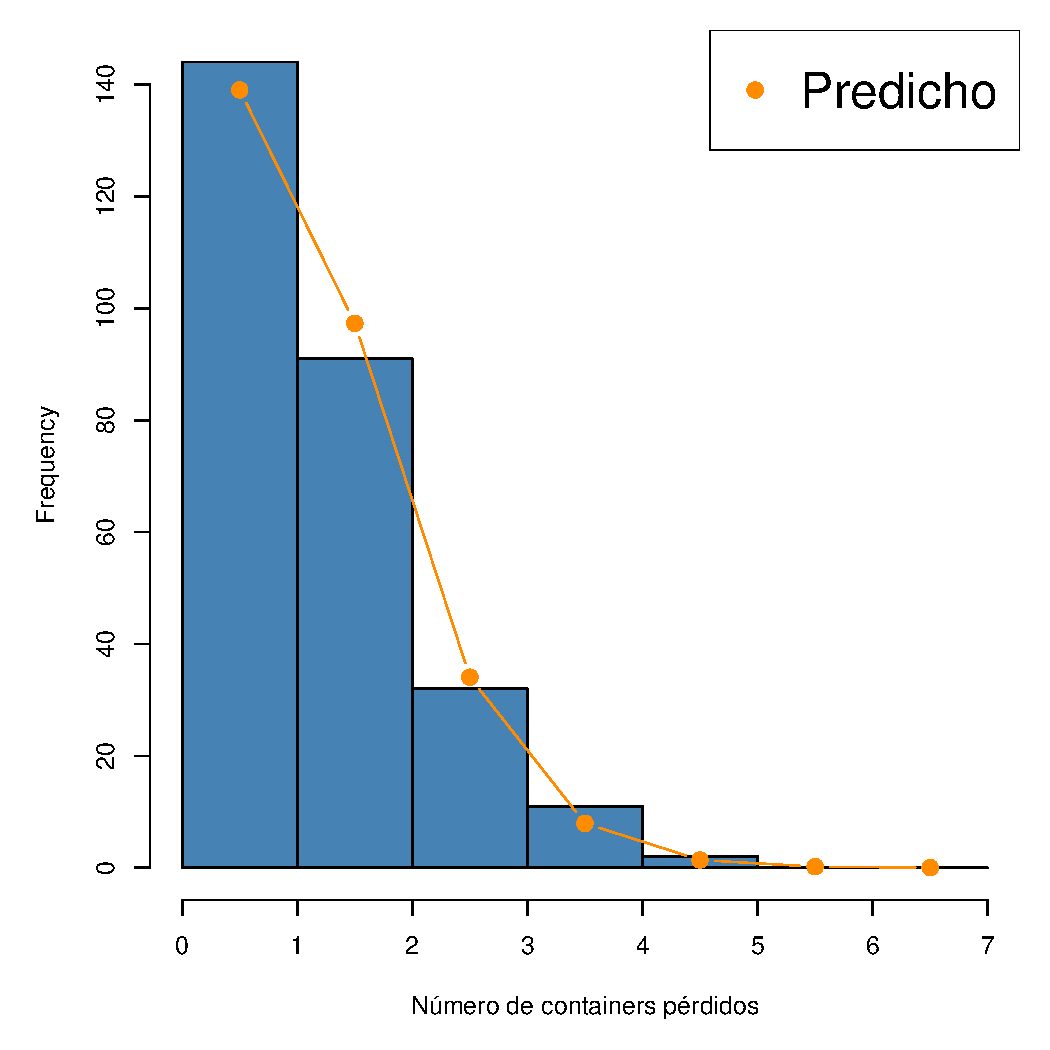
\includegraphics[height=.8\textheight]{slides3/img/hist-soldados-poisson.pdf}
      \end{figure}
    \end{column}
    \begin{column}{.4\textwidth}
     \small Comparamos los datos de containers perdidos graficados en un histograma \color{dodgerblue}(barras azules) \color{black} con la función de probabilidad puntual de una v.a. con distribución Poi(0.7) \color{orang}(puntos naranjas)\color{black}.
      \begin{table}
        \centering
        \begin{tabular}{c| c}
          0& 144\\
          1& 91 \\
          2& 32 \\
          3& 11 \\
          4& 2 \\
          5& 0 \\
          6& 0 \\
          7& 0 
        \end{tabular}
        % \caption{Muertes anuales por patadas de caballo en el
        % ej\'ercito Prusiano (1875-1894)}
      \end{table}
    \end{column}
  \end{columns}
\end{frame}


%\begin{frame}{¿Para qué se puede usar inferencia?}

%\begin{center}
%    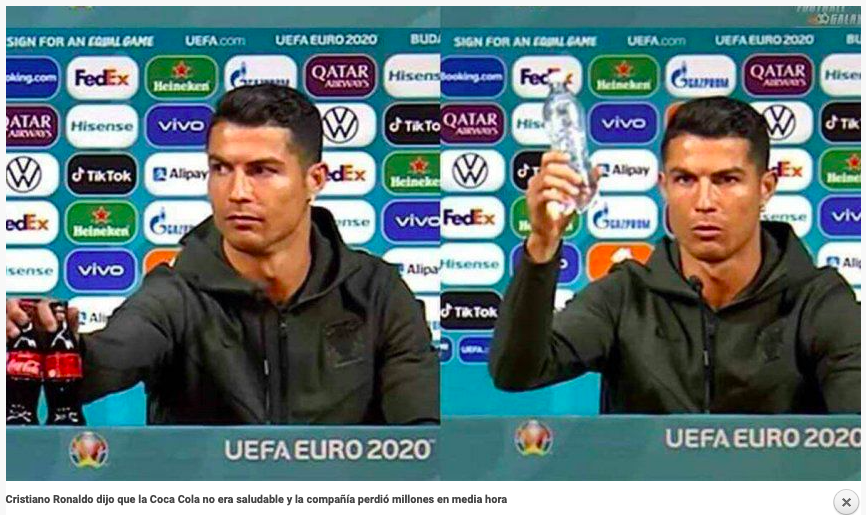
\includegraphics[scale=0.4]{slides1/ronaldo.png}
%\end{center}

%\end{frame}

\begin{frame}{\color{rosee}Introducci\'on a la inferencia estadística}
\small
  \begin{itemize}
\item Las herramientas de inferencia, nos ayudan analizar los datos de para \textbf{tomar decisiones racionales en condiciones de incertidumbre}.\medskip
  \begin{itemize}
  \item ¿Cuántos containers se pierden en promedio por año?
  \item ¿Cuál es la proporción aproximada de containers perdidos por año?

  \end{itemize}
\item Las herramientas de inferencia también nos permiten\textbf{ considerar y cuantificar la incertidumbre} en torno a situaciones inciertas.\medskip
  \begin{itemize}
  \item ¿Cu\'an confiable es la estimaci\'on sobre la proporción de
    containers perdidos por año si dicha estimación está basada en observar durante $20$ años en $16$ centros durante un año?\\
    
  \item ¿De qué depende (y cómo se cuantifica) la confianza en la estimación de la proporción de containers perdidos?
 
  \end{itemize}
    \end{itemize}
\end{frame}


\begin{frame}{\color{rosee}Inferencia estad\'istica}\small
  \begin{block}{}
    El objetivo de la \textbf{inferencia estad\'istica} es sacar conclusiones y/o
    tomar decisiones concernientes a alg\'un par\'ametro desconocido
    bas\'andose s\'olo en los datos de una muestra. A grandes rasgos hay
    tres tipos de \textbf{inferencias} que podemos realizar. Por ejemplo, a partir del ejemplo de los containers perdidos (esto lo haremos para cada ejemplo en la materia)
    
    \begin{enumerate}
    \item \color{blue}\textbf{\underline{estimaci\'on} puntual:} \color{black}dar un valor ``razonable'' (que concuerde con la evidencia empírica) al parámetro desconocido $\lambda:=E(X)$.\footnote{En este caso el parámetro de inter\'es es la cantidad promedio de containers perdidos, para otros ejemplos leer \S14.}
    \item \color{red}\textbf{\underline{estimaci\'on} por intervalos:} \color{black}proveer un intervalo aleatorio $[A,B]$ que, ``con alta confianza'', contenga (cubra) al valor desconocido del parámetro $\lambda$.
    \item \color{deepyellow}\textbf{\underline{test} de hip\'otesis:} \color{black} evaluar la evidencia en contra
      de la hip\'otesis (conjetura) que involucra al (a los) parámetro(s) desconocido(s) el modelo asociado(s) a $X$. Por ejemplo, $H_0: \lambda \leqslant 2$.
    \end{enumerate}
  \end{block}
  
  
A tener en cuenta: ``All models are wrong, but some are useful''. (G. Box)
\end{frame}
\begin{frame}[fragile]{\color{rosee}Estimaci\'on, muestreo y tests}

% bajo algunos environment el & ampersand no se activa y por eso hay que poner fragile en el begin frame. 

%https://tex.stackexchange.com/questions/15093/single-ampersand-used-with-wrong-catcode-error-using-tikz-matrix-in-beamer

%https://tex.stackexchange.com/questions/515697/how-can-we-change-the-positions-of-the-labels-on-a-tikz-cd-commutative-diagram

%https://tex.stackexchange.com/questions/460272/how-to-modify-a-tikz-cd-diagram-by-changing-the-placement-and-length-of-arrows 
\renewcommand{\arraystretch}{1}
\begin{center}
\begin{tikzcd}[column sep=50pt,row sep=50pt]
\begin{array}{c}
 \text{población +}      \\
     \text{modelo estadístico } \textbf{(4)} 
\end{array}
 \arrow{r}{\text{muestreo}} \arrow{rd}{\hspace{-2em}{\begin{array}{c}\text{datos obs.}\munderbar{x}\\ \text{(muestra)} \end{array} }} & {\begin{array}{c} \text{ muestra de datos }\\
     \text{aleatorios } \munderbar{X} \textbf{ (1)}
\end{array}}  \arrow[]{d}{\text{reducción de datos}} \\
 {\begin{array}{c}
\text{\color{blue}est. puntual, \color{red}IC}\\ \text{o \color{deepyellow}comportamiento}\textbf{ (3)} \end{array}} \arrow{u}{\text{inferencia}}  & 
{\begin{array}{c}
\text{\color{blue}esta\color{red}dís\color{deepyellow}tico} \\ \text{\color{blue}estimador} \textbf{ (2)}\end{array}}
 \arrow{l}{{\begin{array}{c}
    \text{\color{blue}estim\color{red}ación \color{black} y/o}\\
    \text{\color{deepyellow} decisión} 
\end{array}}}
\end{tikzcd}
\end{center}


%\begin{center}
%\begin{tikzcd}
%\begin{array}{c}
% \text{población +}      \\
%     \text{modelo estadístico } 
%\end{array}
% \arrow{r}{\text{muestreo}} \arrow{rd}{\hspace{-2em}{\begin{array}{c}\text{datos obs.}\munderbar{x}\\[-12pt] \text{(muestra)} \end{array} }} & {\begin{array}{c} \text{ muestra de datos }\\
%     \text{aleatorios } \munderbar{X} 
%\end{array}}  \arrow[]{d}{\text{reducción de datos}} \\
% {\begin{array}{c}
%\text{\color{blue}est. puntual, \color{red}IC}\\ \text{o \color{deepyellow}comportamiento} \end{array}} \arrow{u}{\text{inferencia}}  & 
%{\text{\color{blue}esta\color{red}dís\color{deepyellow}tico}}
% \arrow{l}{{\begin{array}{c}
    %\text{\color{blue}estim\color{red}ación \color{black} y/o}\\[-12pt] 
%    \text{\color{deepyellow}regla de decisión} 
%\end{array}}}
%\end{tikzcd}
%\end{center}
  
     \begin{itemize}
\item\small{ \textbf{Modelo estadístico}: Colección de distribuciones de probabilidad (y sus \textbf{parámetros}) con las que describimos el comportamiento de v.a. $\{X_i\}_{i=1}^{n}$}\medskip

\item  \small{A partir de datos obtenemos una \textbf{estimación} para un parámetro mientras que a partir de un muestreo aleatorio obtenemos un \textbf{estimador} del parámetro.}\medskip
%\item \small{Podemos pensar en las estimaciones como maneras de combinar de forma oportuna la información que hay en los datos para estimar de forma razonable ciertos parámetros de interés de la población.}
  \end{itemize}

\end{frame}


\begin{frame}{\color{rosee} 1. Muestreo y tipos de inferencia}
    

    \begin{block}{Muestreo, ¿Cómo se realiza?}
          \begin{itemize}
    \item Es importantísimo conocer cómo fue realizado el \textbf{muestreo} a la hora de colectar los datos.
        \item En la materia vamos a asumir que los datos $\munderbar{X}$ son tomados de una \textbf{muestra aleatoria} de tamaño $n$, es decir, que las variables aleatorias $X_1,\cdots, X_n$ son \textbf{independientes e idénticamente distribuidas}. 
     
         \noindent Se escribe: $X_i \sim_{iid}f_X(x;\theta)$ con $i=1,\cdots, n$.\footnotemark
           \end{itemize}
        \end{block}
    
        
        \begin{block}{Tipos de Inferencia}
       \begin{itemize}
        
        \item \underline{\textbf{frecuentista}} o \textbf{bayesiana}.
        \item \underline{\textbf{parámetrica}}, \textbf{semi-paramétrica} y \textbf{no paramétrica}.
        \item En la materia vamos a hacer inferencia \textbf{frecuentista} y, en general, inferencia \textbf{paramétrica}.
        \end{itemize}
        \end{block}
        \footnotetext{Notar que hay algunos resultados (no todos) que vamos a ver en la materia que valen incluso para casos en donde la muestra $\munderbar{X}$ no es iid.}
    
\end{frame}


\begin{frame}{\color{rosee}Ejemplos de parámetros que queremos estimar}
\small
En general nos va a interesar estimar parámetros como: 
    $E(X)$, $Var(X)$, $P(X>0)$, m\'aximo valor de una variable $X$. Por ejemplo:
 \begin{itemize}
 \item \color{gren}Retorno esperado: \color{black}
    Sea $X$ la variable aleatoria que representa el retorno diario de cierto activo financiero. Un par\'ametro de inter\'es aqu\'i es $E(X)$, el retorno esperado. Tambi\'en nos puede interesar estimar
    $Var(X)$ (si existe...), como una medida del riesgo del activo, o $P(X>0)$ que es la probabilidad de un retorno positivo.
     \item\color{gren} Distribuci\'on de la riqueza: \color{black}
    Elegimos una persona al azar de la poblaci\'on adulta de Buenos
    Aires. Sean 1) $X$ su ingreso neto mensual, 2) $F_{X}$ su funci\'on de distribuci\'on acumulada y
    3) $F^{-1}_{X}$ su funci\'on cuantil.

    Un par\'ametro de inter\'es aqu\'i podría ser $q=F^{-1}_{X}(0.9)$
    
    ¿c\'uanto hay que ganar por mes para estar en el $10\%$ m\'as rico?.
    
    \medskip
    También nos podr\'ia interesar (ambiciosamente) toda la funci\'on $F_{X}$!
     \item\color{gren} Tiempo de reacción: \color{black} Nos puede interesar estudiar cuánto es el máximo tiempo que tarda una droga en hacer efecto en pacientes o el máximo tiempo que tarda en reaccionar un auto a una maniobra bajo distintas temperaturas.
  \end{itemize}
  
\end{frame}

\begin{frame}{\color{rosee}2. Reducción de datos: estimadores}
    
        \begin{definition}[Estimador]
   \textbf{Un estimador $\widehat{\theta}_{n} = t(X_1,\cdots, X_n)=t(\munderbar{X}).$ para una función $\beta(\theta)$ de un par\'ametro} $\theta$ (desconocido), es una funci\'on de la muestra aleatoria $\munderbar{X}=\{X_{1},\dots,X_{n}\}$. 

    
  \end{definition}
  
  \vspace{8pt}
      \begin{itemize}
      
        \item \small{\textbf{Un estimador $t(\munderbar{X})$ es una v.a}.} que reduce los datos $\munderbar{X}.$
        \item \small{Un \textbf{valor estimado }$t(\munderbar{x})$ es una realizaci\'on (n\'umero fijo) de un estimador.}
        \item \small{El \textbf{parámetro} $\theta$ es una cantidad fija y desconocida. Por ejemplo, si $X\sim U(a,b)$, $\theta=(a,b)$ y $\beta(\theta)=E(X)=\frac{a+b}{2}$.}
        \item\small{Los estimadores ``reducen la muestra aleatoria'' $\munderbar{X}$ para (idealmente) quedarnos sólo con la información relevante respecto de $\theta$. }
        \item Por ejemplo, un \textbf{estimador para} $E(X)=\frac{a+b}{2}$ si $X\sim U(a,b)$ puede ser $\frac{X_1+X_2+\cdots + X_n}{n}$.
        \item Por ejemplo, un \textbf{estimador para} $b$ (el valor máximo del soporte de las v.a. $X_i$ si $X\sim U(a,b)$ puede ser $\max \{X_1,X_2,\cdots , X_n\}$.
    \end{itemize}
 % \begin{columns}
 % \begin{column}{8cm}
  %  \begin{itemize}
      
   %     \item \small{\textbf{Un estimador $t(\munderbar{X})$ es una v.a}.}
    %    \item \small{Un \textbf{valor estimado }$t(\munderbar{x})$ es una realizaci\'on (n\'umero fijo) de un estimador.}
     %   \item \small{El \textbf{parámetro} $\theta$ es una cantidad fija y desconocida. Por ejemplo, si $X\sim U(a,b)$, $\theta=(a,b)$ y $\beta(\theta)=E(X)=\frac{a+b}{2}$.}
      %  \item\small{Los estimadores ``reducen la muestra aleatoria'' $\munderbar{X}$ para (idealmente) quedarnos sólo con la información relevante respecto de $\theta$. }
    %\end{itemize}
%    \end{column}
 %\begin{column}{6cm}   
  %  $\quad$
   %     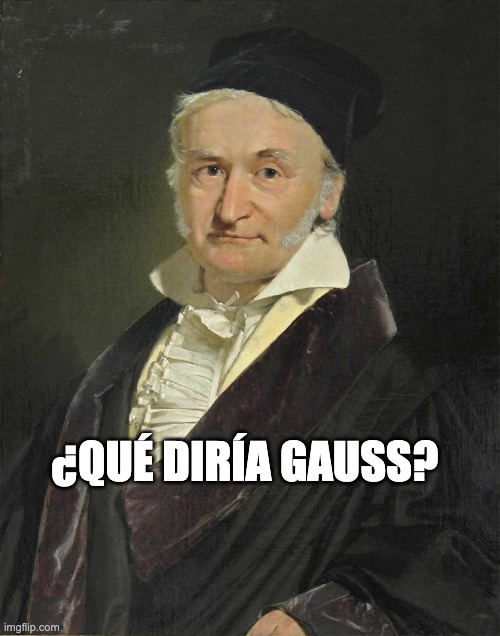
\includegraphics[scale=0.2]{slides1/quediriagauss.jpeg}
    
    %\end{column}
    %\end{columns}
\end{frame}




%\begin{frame}{Ejemplos II (sólo un poco más complicados)}
%    \begin{itemize}
%\item Nos interesa $\theta = E(X^2)$ con $X\sim N(\mu, \sigma^2)$.
%\item Consideremos $\{X_1,\cdots, X_n \} \sim_{iid} \text{N}(\mu,\sigma^2)$ y $t_2(\munderbar{X})=\dfrac{1}{n}\displaystyle\sum_{i=1}^{n}X_i^2$.
%\item A cada realización de la muestra aleatoria (para cada conjunto de datos), corresponderá una estimación diferente de $\theta$ (¿qué intuyes va a ocurrir con las diferentes realizaciones de $t_2$ cuando $\sigma$ es muy pequeño? y en caso contrario?).\bigskip

%\item Sabemos/asumimos que $X\sim \text{Unif}(0, \theta)$ y nos interesa  \textbf{estimar} $\theta$.
%\item  Consideremos $\{X_1,\cdots, X_n \} \sim_{iid} \text{Unif}(0, \theta)$ y el estimador $t_3(\munderbar{X})=\max\{X_1,\cdots, X_n \}$ (¿porqué tiene sentido este estimador?).
%\item A cada realización de la muestra aleatoria (para cada conjunto de datos), corresponderá una estimación diferente de $\theta$ (¿qué intuyes va a ocurrir con las realizaciones de $t_3$ cuando $n$ sea extremadamente grande? y en caso contrario?).\bigskip
%    \end{itemize}
%\end{frame}



\begin{frame}{\color{rosee}2. Ejemplos de estimadores}
\small
    
    \begin{table}[h!]
        \centering
        \begin{tabularx}{\linewidth}{|>{\hsize=0.6\hsize}X|>{\hsize=1.18\hsize}X|>{\hsize=1.23\hsize}X|}
        \hline
     $\beta(\theta)$ &  estimador $t(\munderbar{X})$ & modelo estadístico \\
         \hline
      $E(X)=\theta$ & $\dfrac{1}{n}\displaystyle\sum_{i=1}^{n}X_i:=\overline{X}_n$  &$X_i \sim_{iid} Ber(\theta)$\\
      \hline
  \scalebox{0.8}{$ E(X^2)=\theta^2+\sigma^2$}  &$\dfrac{1}{n}\displaystyle\sum_{i=1}^{n}X_i^2$ &\scalebox{0.9}{$X_i \sim_{iid} N(\theta,\sigma^2)$}, $\sigma$ \small{conocido}\\
     \hline
   \scalebox{0.9}{$Var(X)=\theta^2$}   & \scalebox{0.9}{$S^2:=\dfrac{1}{n-1}\displaystyle\sum_{i=1}^{n}\left(X_i-\overline{X}_n\right)^2$} &\scalebox{0.9}{$X_i \sim_{iid} N(\mu,\theta^2)$}, $\mu$ \small{conocida}\\
     \hline
    \small{\textbf{máximo valor} $\theta$ del soporte de las v.a. $X_i$} & $\max\{X_1,X_2,\cdots,X_n\}$ o, por ejemplo, $2\overline{X}_n$ & $X_i \sim_{iid} U(0,\theta]$\\
     \hline
      \end{tabularx}
       \end{table}
       
    \begin{itemize}
        \item Se conoce a $\overline{X}_n$ como la \textbf{media muestral}.
        \item Se conoce a $S^2$ como la  \textbf{varianza muestral}.
    \end{itemize}
    Durante las primeras clases nos vamos a concentrar en el parámetro $E(X)$ y vamos a usar el estimador media muestral $\overline{X}_n$.
\end{frame}


\begin{frame}{\color{rosee}Ejemplo I de todos los pasos del diagrama}
\small
    \begin{itemize}
\item  Imaginamos que nos interesa estudiar la proporci\'on de la poblaci\'on estuvo enferma en alg\'un momento del COVID-19 en los adultos de Argentina (nuestra población de interés).\medskip

\item Llamemos $X$ a la variable aleatoria que asume valor $1$ cuando la persona $i$-\'esima que est\'a por ser elegida al azar contrajo en algún momento la enfermedad y $0$ en otro caso.\medskip

\item Nos interesa estimar $\theta \equiv E(X)$ (\textbf{proporción poblacional}).\medskip

\item Resulta razonable asumir que $X\sim \text{Be}(\theta)$ (¿porqué?).\bigskip

\item Muestra aleatoria: $X_1,\cdots, X_n  \sim_{iid} \text{Be}(\theta)$.  
\item Estimador $t_1(\munderbar{X})=\dfrac{1}{n}\displaystyle\sum_{i=1}^{n}X_i=\overline{X}_n$ (¿cómo se distribuye $t_1$?).\medskip 
\item Datos si $n=5$:  {\small $\munderbar{x}=(X_1=1,X_2=0,X_3=0,X_4=1, X_5=0 )$}. 
\item Estimación puntual de $\theta$: $t_1(\munderbar{x})=\dfrac{2}{5}$. ¿Qué tan precisa es?
    \end{itemize}
\end{frame}

\begin{frame}{\color{rosee}2. Propiedades de estimadores} \small 


Nos interesa entender qu\'e propiedades tienen los
  estimadores de ciertos parámetros de interés $\beta(\theta)$ para responder, entre  otras, las siguientes preguntas:
  \begin{itemize}
  \item Siendo $t(\munderbar{X})$ una variable aleatoria, me gustaría saber si por ejemplo $E(t(\munderbar{X}))=\beta(\theta)$ (en promedio el estimador estima el valor $\beta(\theta)$.\medskip
  \item ¿Cómo se distribuye $t(\munderbar{X})$? ¿Puedo garantizar que, con alta probabilidad, el estimador va  a tomar valores \textbf{cercanos} al del valor verdadero (fijo y desconocido) del parámetro que  queremos estimar?\medskip
  \item ¿C\'omo definimos si un estimador es ``\textbf{mejor}'' que otro?  ¿Existe un estimador que sea \textbf{\'optimo} a la hora de estimar un cierto par\'ametro desconocido?\medskip

  \item ¿Cu\'antas (y qu\'e tipo de) observaciones necesitamos para
    garantizar cierto \textbf{margen de error} con probabilidad alta?
  \end{itemize}

En la mayoría de los casos, s\'olo vamos a poder dar
  respuestas aproximadas, basadas en
  resultados \textbf{asint\'oticos} (cuando $n\to \infty$/ con $n\gg 0$ en la práctica).
  
 % Nos interesa entender qu\'e propiedades tienen distintos estimadores de distintos par\'ametros para responder, entre otras, las siguientes preguntas:
 % \begin{itemize}
 % \item ¿Qu\'e propiedades tiene la \textbf{distribuci\'on muestral} del
  %  estimador?
  %\item ¿C\'omo medimos si un estimador es \textbf{mejor} que otro? ¿C\'ual es la manera \textbf{\'optima} de estimar un par\'ametro?
  %\item ¿Podemos garantizar que, con mucha probabilidad, el estimador va
   % a estar \textbf{cerca} del valor verdadero (fijo y desconocido) que
%    queremos estimar?
 % \item ¿Cu\'antas (y qu\'e tipo de) observaciones necesitamos para
  %  garantizar cierto \textbf{margen de error} con probabilidad alta?
  %\end{itemize}

  %Para la mayor\'ia de los problemas, s\'olo vamos a poder dar respuestas aproximadas a estas preguntas, basadas en resultados \textbf{asint\'oticos} (con un n\'umero de observaciones que
%  tiende a infinito).


\end{frame}

\begin{frame}{\color{rosee}Media muestral  $\overline{X}_n$ y distribuci\'on muestral}
\small
  \begin{alertblock}{\color{rosee}Primer estimador que consideramos:}
      Queremos 
    \textbf{estimar la esperanza/media poblacional $\beta(\theta)=E(X)$ de la v.a. $X$ usando la media muestral $\overline{X}_n$}. 
  \end{alertblock}

  \begin{block}{La media muestra es una variable aleatoria}
    Dada una muestra aleatoria $X_{1},\dots,X_{n}$, la media muestral
    \begin{equation*}
      \overline{X}_{n}=\frac{X_{1}+\dots+X_{n}}{n}
    \end{equation*}
    es una variable aleatoria y por lo tanto tiene su propia
    distribuci\'on.
  \end{block}



\end{frame}

\begin{frame}{\color{rosee}Distribución muestral de $\overline{X}_n$ - ejemplos}\small
    Si $X_i\sim_{iid}$ entonces $n\overline{X}_n=\displaystyle\sum_{i=1}^{n}X_i$ se distribuye:
    \begin{table}[h!]
        \centering
        \begin{tabularx}{\linewidth}{|>{\hsize=0.6\hsize}X|>{\hsize=1.4\hsize}X|}
        \hline
        \textbf{Modelo estadístico}& \textbf{Distribución de} $n\overline{X}_n$\\
        \hline
        $X\sim_{iid}Be(p)$ & $n\overline{X}_n\sim Bi(n,p)$\\
        \hline
          $X\sim_{iid}N(\mu,\sigma^2)$ & $n\overline{X}_n\sim N(n\mu,n\sigma^2)\Rightarrow \overline{X}_n\sim N\left(\mu,\frac{\sigma^2}{n}\right)$\\
        \hline  
        $X\sim_{iid}U(0,\theta)$ & $\frac{n\overline{X}_n}{\theta} \sim \text{Irwin-Hall}$\\
        \hline
          $X\sim_{iid}Exp(\theta)$ & $n\overline{X}_n \sim \Gamma(n,\theta)$\\
        \hline
        \end{tabularx}
        \end{table}
\end{frame}

%\begin{frame}{\color{rosee} Actividad (parte 1 de 3)}
%\begin{itemize}
 %   \item    \textbf{Para enfatizar que} $\overline{X}_n$ \textbf{es una variable aleatoria}, \textbf{analizar qué forma tiene la distribución muestral y remarcar cuál es la diferencia entre la estimación $\overline{x}_n$ y el estimador $\overline{X}_n$} vamos a realizar la siguiente actividad. 
    
  %  \item Consideramos $X_i$ la cantidad de likes del post $i$-ésimo que postea Billie Eilish. ¿Qué representa la v.a. $\overline{X}_n$? ¿Cuál es el \textbf{soporte} de (posibles valores $x$ que toman) las variables $X_i$ y $\overline{X}_n$? 
    
   % \item Supongamos que queremos estimar $E(X)$. ¿Por qué podríamos argumentar que para estimar $E(X)$ es razonable utilizar al estimador $\overline{X}_n$?
    
    %\item ¿Cómo definimos una muestra aleatoria en este contexto? ¿Bajo qué condiciones experimentales podemos decir que $\{X_1,\cdots, X_n\}$ son v.a.i.i.d.?
   
    
   % \item \textbf{Pregunta extra:} Si $Y_i$ representa la cantidad de likes en el post i-ésimo que postea B.E. en las primeras 24 hs ¿qué modelo estadístico resulta razonable para $Y$?
    
 %   \end{itemize}
  %  \end{frame}
  
 % \begin{frame}{\color{rosee} Actividad (parte 2 de 3)} 
  
 % Hacé click en el siguiente link para completar en las filas A y B en \href{https://docs.google.com/spreadsheets/d/16g9d3e6sTJLrZvEQhvQvhGYG1k_j7DOE7fxyg9xbKTY/edit?usp=sharing}{Google form Billie Eilish}. Tenés que hacer lo siguiente:
  
 %   \begin{enumerate}
  %      \item \textbf{Si tenés apellido de la A a la H} buscá 2 (5) posts viejos en IG de Billie Eilish y calculá $\overline{x}_2$ ($\overline{x}_{5}$).
   %     \item \textbf{Si tenés apellido de la I a la Q} buscá 2 (5) posts, algunos viejos y otros nuevos en IG de Billie Eilish y calculá $\overline{x}_2$ ($\overline{x}_{5}$).
    %    \item \textbf{Si tenés apellido de la R a la Z} buscá 2 (5) posts nuevos en IG de Billie Eilish y calculá $\overline{x}_2$ ($\overline{x}_{5}$).
%    \end{enumerate}
 % \begin{itemize}  
  %  \item Notá que si el promedio de likes te da 1.234.567 entonces tenés que escribir $1,23$ en la celda correspondiente.
   % \item ¿Qué diferencias podés notar entre la distribución muestral de $\overline{X}_2$ y la de $\overline{X}_{5}$?
%    \end{itemize}
 %   \end{frame}
    
 %     \begin{frame}{\color{rosee} Actividad (parte 3 de 3)} 
  %        \begin{itemize}
   % \item Veamos el histograma de likes y \textbf{estimemos la media poblacional} $E(X)$.  \href{https://thesocialflame.com/en/influencer/billieeilish}{Ver the social flame}
    %    \end{itemize}
        
     %   \begin{center}
      %      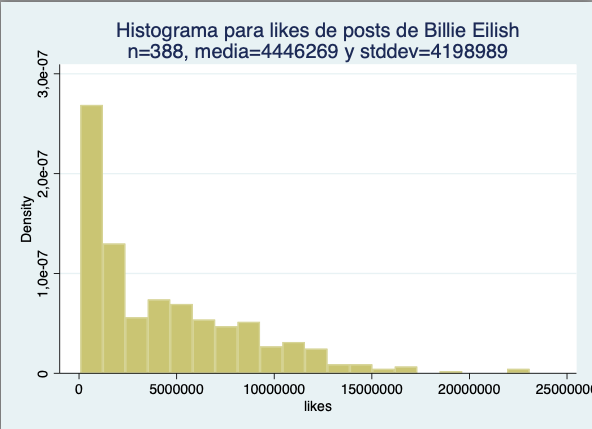
\includegraphics[scale=0.4]{slides1/be.png}
       % \end{center}
%\end{frame}



%\begin{frame}[fragile]{\color{rosee}Distribuci\'on muestral}\small
%  \begin{lstlisting}
%    library(animation)
%    saveHTML({
%    for (iter in seq(10, 500, 5)) {
%        n_muestra <- iter
%        param <- 0.7
%        ## Generamos 1000 muestras
%        muestras <- replicate(n = 1000,
%                              rbinom(n = iter, 
%                                     size = 1, 
%                                     prob = parametro))
%        ## Calculamos la media de cada muestra
%        medias <- colMeans(muestras)
%        ## Graficamos el histograma
%        hist(medias, freq = FALSE, breaks = iter/5,
%             main = paste("Histograma, n=", iter),
%             xlab = "Medias muestrales", 
%             col = "steelblue", lwd = 3, density = 45,
%             xlim = c(0, 1))#, ylim = c(0, 15))
%        abline(v = param, col = "darkorange", lwd = 3)
%      }})
%  \end{lstlisting}
%\end{frame}


\begin{frame}{\color{rosee}Propiedades de la media muestral}\small
 % En la siguiente proposici\'on, formalizamos algo que ya hab\'iamos notado en las simulaciones con R.
 
 Considerando una \textbf{muestra aleatoria} $\munderbar{X}$, es decir los datos $X_i\stackrel{iid}{\sim}$ ,
  \begin{block}{}
    si existe $E(X)$, entonces como los datos $X_i$ son idénticamente distribuidos (no hace falta asumir independencia)
    \begin{equation*}
      E\left(\overline{X}_{n} \right) = E(X).
    \end{equation*}
    si existe $Var(X)$, entonces como los datos $X_i$ son independientes e idénticamente distribuidos 
    
    \begin{equation*}
      \quad Var(\overline{X}_{n} )=\frac{Var(X)}{n}.
    \end{equation*}
  \end{block}

   
  \begin{itemize}
   \item La distribuci\'on de $\overline{X}_{n}$ est\'a centrada en $E(X)$ y
    su varianza disminuye (¿por qué? \href{https://www.npr.org/sections/money/2015/08/07/429720443/17-205-people-guessed-the-weight-of-a-cow-heres-how-they-did}{ver historia vaca}) a medida que aumenta el
    tama\~no de la muestra.
    %\shrug %\begin{verbatim}¯\_(ツ)_/¯\end{verbatim}
  \end{itemize}
\end{frame}

\begin{frame}{\color{rosee}Propiedades de la media muestral - demostración} \small
    \begin{itemize}
    \item Usamos la linealidad de la esperanza y que los datos $X_i\stackrel{id}{\sim}$ (notar que NO usamos independencia en este caso)
    \end{itemize}
      \begin{align*}
        E\left(\overline{X}_{n} \right) 
        &= E\left(\frac{1}{n}\sum\limits_{i=1}^{n}X_{i} \right)\underbrace{=}_{lin. \, E}
          \frac{1}{n}E\left(\sum\limits_{i=1}^{n}X_{i} \right) \\
        &\underbrace{=}_{lin. \, E}\frac{1}{n}\sum\limits_{i=1}^{n}E\left( X_{i}\right)\underbrace{=}_{X_i \text{ id}} \frac{1}{n} n E(X) =E(X)
      \end{align*}
    \begin{itemize}
    \item Con las propiedades de la varianza y que los datos $X_i\stackrel{iid}{\sim}$ (notar que S\'I usamos independencia en este caso)
      \begin{align*}
        Var\left(\overline{X}_{n} \right) 
        &= Var\left(\frac{1}{n}\sum\limits_{i=1}^{n}X_{i} \right)
          \underbrace{=}_{cons^2}\frac{1}{n^2}Var\left(\sum\limits_{i=1}^{n}X_{i} \right)\\ 
        &\underbrace{=}_{X_i \text{ indep}}\frac{1}{n^2}\sum\limits_{i=1}^{n}Var\left( X_{i}\right)
          \underbrace{=}_{X_i \text{ id}} \frac{1}{n^{2}} n Var(X)=\frac{Var(X)}{n}
      \end{align*}
    \end{itemize}
    \vskip-0.2cm
  
\end{frame}

\begin{frame}{\color{rosee} Actividad en clase: ejemplo 1}\small
Para enfatizar que $\overline{X}_n$ es una \textbf{variable aleatoria}, analicemos qué forma tiene su distribución muestral y remarquemos las diferencia entre el estimador $\overline{X}_n$ y la estimación $\overline{x}_n$,  vamos a realizar la siguiente actividad:\medskip
\begin{itemize}
    \item Consideramos las v.a. $X_i$ que toman valor $1$ cuando tiramos una moneda y sale cara (escudo) y 0 cuando sale cruz (número, ceca) en la tirada $i$-\'esima.\medskip
    \item ¿Qué modelo estadístico resulta razonable para las $X_i$? 
    \item  ¿Cuánto estimás que vale el parámetro $\theta = E(X)$ según los datos que recopilaste?\medskip  
    
    \item ¿Cómo definimos una ``muestra'' aleatoria en este contexto? ¿Bajo que condiciones experimentales podemos decir que $\{X_1,\dots,X_n\}$ son variables aleatorias independientes e idénticamente distribuidas?\medskip
    
  \item  Ten\'e a mano tu moneda y hac\'e click \href{https://docs.google.com/spreadsheets/d/1Xk34raiH3NqPtKeNKvnyUuBCSnd62Z8W311ljPjD0j8/edit?usp=sharing}{en el enlace}. Si no tenés monedas usá \href{https://www.random.org/coins/}{este link} para hacer el experimento online. %Acá están los resultados del \href{https://docs.google.com/spreadsheets/d/1F_dN9wNL3T5nu8RgLsUjlgrpVz_Zr1FdGHaJDNG2rzc/edit?usp=sharing}{año pasado}.
  % link de 2do semestre 2022
  %https://docs.google.com/spreadsheets/d/13465hxlPmINFVkSI4sXIw0IoMY71rBaBmsrM5WxtcZw/edit?usp=sharing
 % \item ¿Otro ejemplo en \texttt{R}? (Codigo2.R)
    \end{itemize}
    \end{frame}

%\begin{frame}{\color{rosee}Inferencia estad\'istica}\small

%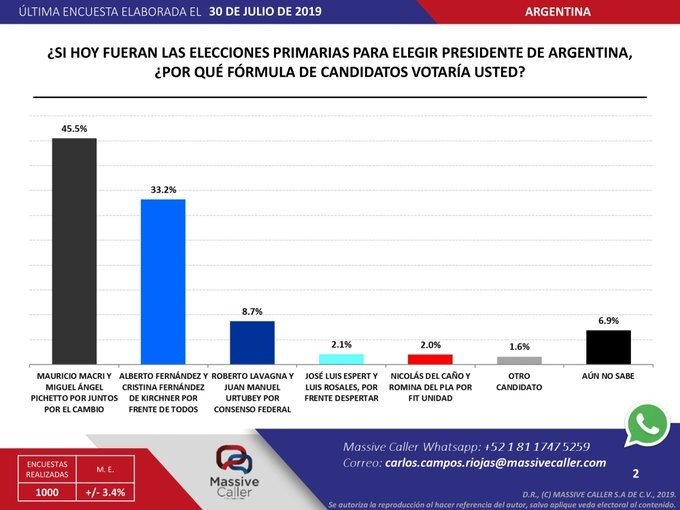
\includegraphics[scale=0.43]{slides1/encuesta.jpeg} 
%\end{frame}

%\section{Estimaci\'on puntual}



\begin{frame}{\color{rosee}3. Estimaci\'on puntual de $E(X)$ usando $\overline{X}_n$: ejemplo 2} 

  \begin{block}{Problema de estimaci\'on puntual}\small
\small{Queremos estimar \textbf{un par\'ametro} $\theta$ asociado a
    una variable aleatoria de inter\'es $X$}.
  \end{block}

 

  \small{Nos interesa estudiar el  \href{https://www.businessinsider.com/smartphone-adoption-on-the-upswing-in-nigeria-2017-4}{grado de adopción/uso de los \textit{smartphone} en Nigeria}. Nos interesará considerar la distribución de una variable $X_i$ en la poblaci\'on de adultos nigerianos.

   \begin{equation*}
    X_{i} =\begin{cases}
      1 & \text{si la i-\'esima persona en Nigeria tiene un smartphone}\\
      0 & \text{si la i-\'esima persona en Nigeria no tiene un smartphone}
    \end{cases}
    \end{equation*}
    
  Es razonable pensar que $X_i\stackrel{iid}{\sim} \text{Bern}(p)$, donde $p=E(X)$ será nuestro parámetro de interés (el grado de adopción de smartphones).}
  
 \small{Notemos que $\theta=p$ \textbf{es un n\'umero fijo y desconocido.} ¿Qué representa $p$ en este modelo estadístico}?
  

%  \item
%    \href{https://www.researchgate.net/publication/277787128_Mobile_Banking_Adoption_in_Nigeria}{Mobile
%      Banking Adoption in Nigeria}
%  \item
%    \href{https://www.utupub.fi/bitstream/handle/10024/143973/Chukwumah\%20Samuel.pdf?sequence=1}{Adoption
%      of mobile banking service in rural Nigeria (Master Thesis).}
  
  % \cite{bankole2011mobile}

\end{frame}


\begin{frame}[fragile]{\color{rosee}3. Estimaci\'on puntual de $E(X)$ usando $\overline{X}_n$: ejemplo 2} 
  
 \small{Supongamos que, para el ejemplo de los \textit{smartphones}, le preguntamos a 10 habitantes nigerianos si tienen smartphone o no y obtuvimos
  las siguientes mediciones}
  \[x_{1},\dots, x_{10}\]
 \noindent \small{ obtenidas todas que obtuvimos eligiendo $10$ personas al \textit{azar}.}

  \medskip
  \begin{table}
    \centering
    \begin{tabular}{c|c|c|c|c|c|c|c|c|c}
      \specialrule{.2em}{.2em}{.2em}
      1 & 2 & 3 & 4 & 5 & 6 & 7 & 8 & 9 & 10 \\
      \hline
      1 & 1 & 1 & 0 & 1 & 0 & 0 & 0 & 1 & \phantom{-}1\\
      \specialrule{.2em}{.2em}{.2em}
    \end{tabular}
    %\caption{$10$ mediciones al azar para el ejemplo de los \textit{smartphones}.}
    \label{tab:smartphones}
  \end{table}
   
  Con estos datos, queremos construir una estimaci\'on del
  par\'ametro $p$ como:
  \begin{equation*}
    \frac{x_{1}+x_{2}+\dots+x_{10}}{10}= 0.6
  \end{equation*}
  \begin{lstlisting}
    ## En R:
    set.seed(seed = 1)  # para que sea reproducible
    muestra = rbinom(n = 10, size = 1, prob = 0.65)
    mean(muestra)  # calculamos el valor de la estimacion
  \end{lstlisting}
\end{frame}

\begin{frame}{\color{rosee} $\overline{x}_n$ estimaci\'on puntual de $E(X)$ vs. estimador $\overline{X}_n$ de $E(X)$} \small
\begin{itemize}
    \item  La estimación puntual de $p$ usando los datos observados $\munderbar{x}=(1,1,1,0,1,0,0,0,1,1)$ es
  \begin{equation*}
    \frac{x_{1}+x_{2}+\dots+x_{10}}{10}=0.6.
  \end{equation*}

    \item Observemos que para cada muestra particular $\munderbar{x}$ $\overline{x}_{10}$ es un número.
    \item Notemos tambi\'en que si repitiéramos el experimento y fueran
    seleccionadas otras personas nuestro valor estimado podr\'ia
    cambiar. Por eso $\overline{X}_n$ es una v.a.
    \item  Nuestras mediciones (datos) $x_{1},\dots, x_{10}$ son
  \textbf{realizaciones} de variables aleatorias $X_{1},\dots, X_{10}$ son variables iid.
   \item \small{Para una muestra aleatoria el estimador media muestral verifica que $E\left(\overline{X}_{n} \right) =E(X)$ y $Var(\overline{X}_{n} )=\frac{Var(X)}{n}$. Luego, $\overline{X}_{n}$  parece una herramienta adecuada para inferir sobre $E(X)$ ¿por qué?.} \medskip
  %\item \small{A continuación, discutimos cómo estimar $p$ con datos.}
  \item Consideramos a la media muestral $\overline{X}_n$ es un \textbf{estimador} de $p$.
  \item \textbf{Notaci\'on}:
    Usamos\textbf{ min\'usculas} para \textbf{n\'umeros fijos}, \textbf{may\'usculas }para\textbf{ variables
    aleatorias}.
\end{itemize}

 % \begin{alertblock}{}
  %  Recordemos que, formalmente, una variable aleatoria es una funci\'on del espacio muestral $\Omega$ a los n\'umeros reales. La relaci\'on entre nuestras mediciones $x_{1},\dots, x_{10}$ (n\'umeros fijos) y las variables aleatorias $X_{1},\dots, X_{10}$ es
%    \begin{equation*}
%      x_{i}=X_{i}(\omega) \quad i=1,\dots,10    
%    \end{equation*}
%    para cierto $\omega\in\Omega$.
 % \end{alertblock}

\end{frame}

\begin{frame}[fragile]{\color{rosee}Media muestral - simulación: ejemplo} \small
  \begin{lstlisting}
    ## En R:
    > set.seed(1)
    > muestras <- replicate(5, rbinom(n=10, 
                                      size=1, 
                                      prob=0.65))
    > muestras
         [,1] [,2] [,3] [,4] [,5]
    [1,]    1    1    0    1    0
    [2,]    1    1    1    1    1
    [3,]    1    0    0    1    0
    [4,]    0    1    1    1    1
    [5,]    1    0    1    0    1
    [6,]    0    1    1    0    0
    [7,]    0    0    1    0    1
    [8,]    0    0    1    1    1
    [9,]    1    1    0    0    0
    [10,]   1    0    1    1    0
    > colMeans(muestras)
    [1] 0.6 0.5 0.7 0.6 0.5
  \end{lstlisting}
\end{frame}


\begin{frame}[fragile]{\color{rosee}Distribuci\'on muestral de $\overline{X}_n$: ¿c\'omo cambia si aumenta $n$?}\small

\begin{table}[]
    \centering
    \begin{tabular}{cc}
  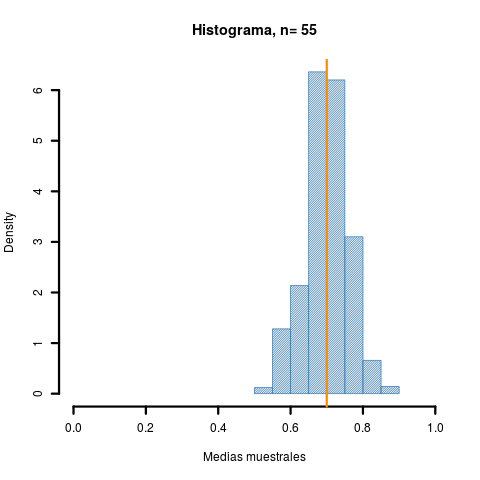
\includegraphics[scale=0.35]{slides1/img/Rplot10.png}       &  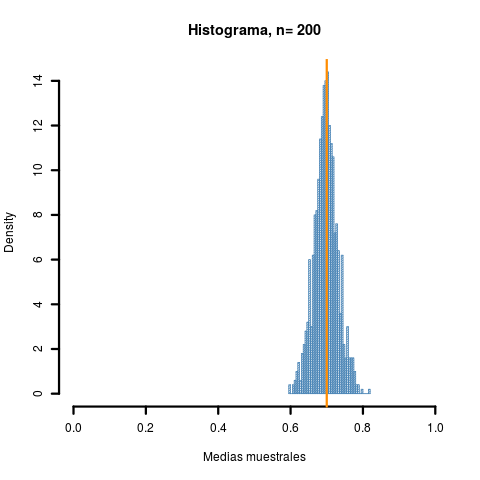
\includegraphics[scale=0.35]{slides1/img/Rplot39.png}   
    \end{tabular}
    \caption{Notemos que a medida que $n$ aumenta, la distribución de $\overline{X}_n$ se concentra alrededor del parámetro $E(X)$ que, para este ejemplo simulado, es 0.7.}
    \label{tab:my_label}
\end{table}
\end{frame}

\begin{frame}[fragile]{\color{rosee}Distribuci\'on muestral de $\overline{X}_n$ para los dos ejemplos}\small
  
  En ambos casos $X_i\stackrel{iid}{\sim}Be(p)$ usando $\overline{X}_n$, el estimador de $p$. Tratemos de pensar cómo se distribuye $\overline{X}_n$ para distintos valores de $n$ y de $p$.
  
 \begin{enumerate}
      \item \textbf{¿Cómo cambia la distribución muestral de $\overline{X}_n$ si cambiamos el parámetro $p$ y mantenemos fijo el tamaño de muestra $n$?  }	
        \begin{itemize}
     \item Para poder responder a esta pregunta, compare qué ocurre cuando $p$ es cercano a 0.5 vs. cuando $p$ es cercano a $0$ o $1$. Tenga en cuenta, usando los resultados de \S21, ser tiene que que $E(\overline{X}_n)=p$ y $Var(\overline{X}_n)=\dfrac{p(1-p)}{n}$.
     \item Sabemos que $n\overline{X}_n \sim Bin(n,p)$ en ese caso la distribución de $\overline{X}_n$ asignará mayor probabilidad a valores cercanos a $p$.
    \end{itemize}
  	
  
    \item \textbf{¿Cómo cambia la distribución muestral de $\overline{X}_n$ si fijamos el parámetro $p$ y aumentamos el
    tama\~no de la muestra $n$?}
     \begin{itemize}
     \item Para poder responder a esta pregunta observe que la varianza de $\overline{X}_n$ disminuye con $n$, es decir, $Var(\overline{X}_n)=\dfrac{p(1-p)}{n}$.
     \item Sabemos que $n\overline{X}_n \sim 
     Bin(n,p)$ en ese caso la distribución de $\overline{X}_n$ estará cada vez más concentrada para valores cercanos a $p$.
    \end{itemize}
    \end{enumerate}
  
\end{frame}

\begin{frame}{\color{rosee}Muestreo vs. simulación de datos}
\small
Si bien en los dos ejemplos colectamos datos $X_i\stackrel{iid}{\sim} Be(p)$, usamos $\overline{X}_n$ como estimador de $p$, ¿qué diferencia a estos ejemplos?

    \begin{itemize}
        \item En el ejemplo de la moneda, para ver cómo era la distribución de las v.a. $X_1+\cdots +X_5$ o $X_1+\cdots +X_{10}$, obtuvimos muestras a partir de \textbf{datos que colectamos}.
        \item En el caso de la adopción de celulares en Nigeria, \textbf{simulamos los datos}. Es decir, a partir de leer en el artículo que aproximadamente un 65\% de la población adopta celulares, simulamos datos que podrían representar esa situación. 
        
        \item ¿Para qué sirve simular datos? Para poder ver cómo se verían datos recopilados si el grado de adopción de smartphones fuese 65\% (u otro porcentaje).
   \end{itemize}
\end{frame}


%\begin{frame}{\color{rosee}Estimadores vs est. puntual, ¿qué estimador elegiríamos?} \small
%  En el ejemplo que ven\'iamos trabajando de los \textit{smartphones}:
%  \begin{align*}
%    \mbox{Estimador:} \quad & \hat{p}_1=\frac{X_{1}+\dots+X_{10}}{10} \\
  %  \mbox{Valor estimado}: \quad & \hat{p}_{1,\text{obs}}=\frac{x_{1}+\dots+x_{10}}{10}= 0.6
  %\end{align*}
  
  %Otro estimador (¿qu\'e opina del estimador?),
  %\begin{align*}
  %  \mbox{Estimador}: \quad &  \hat{p}_2=\frac{X_{1}+X_{2}}{2}\\
  %  \mbox{Valor estimado}: \quad & \hat{p}_{2,\text{obs}}=\frac{x_{1}+x_{2}}{2}=\frac{1 + 1}{2} = 1
  %\end{align*}
  
  %Otro estimador (¿qu\'e opina del estimador?),
  %\begin{align*}
  %  \mbox{Estimador}: \quad &  \hat{p}_3=\dfrac{X_{(5)}+X_{(6)}}{2}\\
  %  \mbox{Valor estimado}: \quad & \hat{p}_{3,\text{obs}}=\frac{x_{(5)}+x_{(6)}}{2}=\frac{1 + 1}{2} = 1
 % \end{align*}
%\end{frame}

%\begin{frame}{\color{rosee}Estimaci\'on puntual: otros ejemplos}
 % \begin{itemize}
  %    \item \color{gren}N\'umero esperado de clientes: \color{black}  Sea $X$ la variable aleatoria que representa el n\'umero de clientes
   % que entran cada d\'ia a un comercio. Un par\'ametro de inter\'es aqu\'i es $E(X)$, el n\'umero de clientes
    %esperado.
    
    %\item \color{gren}Retorno esperado: \color{black}
    %Sea $X$ la variable aleatoria que representa el retorno diario
%de cierto activo financiero. Un par\'ametro de inter\'es aqu\'i es $E(X)$, el retorno
 %   esperado. Tambi\'en nos puede interesar estimar
  %  $Var(X)$ (si existe...), como una medida del riesgo del activo, o $P(X>0)$ que es
   % la probabilidad de un retorno positivo.
%  \end{itemize}
 
  % clientes
%  \begin{itemize}
%  \item\href{https://pdfs.semanticscholar.org/bd76/7c176e1360cf9eca93292cfbca7d6eb6ae5f.pdf}
%    {Perdikaki, O., Kesavan, S., \& Swaminathan, J. M. (2012). Effect of
%      traffic on sales and conversion rates of retail
%      stores. Manufacturing \& Service Operations Management, 14(1),
%      145-162.}
%  \end{itemize}
%\end{frame}


%retorno ejemplo
%  \begin{itemize}
%  \item
%    \href{https://pdfs.semanticscholar.org/fba8/3f0751216eafe5e69da92c61741b06358e82.pdf}
%    {Fryzlewicz, P. (2005). Modelling and forecasting financial
%      log-returns as locally stationary wavelet processes. Journal of
%      Applied Statistics, 32(5), 503.  }
%  \end{itemize}
%\end{frame}

% \begin{frame}{\color{rosee}Estimaci\'on puntual}
%   \begin{example}[Scoring]
%     Para clientes de un banco, sean $X_{1}=$`ingreso mensual',
%     $X_{2}=$`a\~nos de educaci\'on' e $Y$ la variable que vale uno si el
%     cliente devolver\'a el dinero de un pr\'estamo y cero si no.
%   \end{example}
% \end{frame}



%\begin{frame}{\color{rosee}Extra - Para calcular la curva: ¿media o mediana?}
%    \begin{itemize}
%        \item Supongamos que en un curso de $4$ alumnos, $3$ obtienen $30$ puntos de promedio y otro obtiene $100$ de promedio. ¿Cuál es la nota de aprobación si:
        
%        \begin{itemize}
%            \item cada alumno debe obtener al menos de dos tercios de la media?
%         \item cada alumno debe obtener al menos de dos tercios de la mediana?
%        \end{itemize}
        
%        \item ¿Cambiaría su respuesta si hubiese $20$ alumnos en el curso y todos excepto uno hubieran sacado $30$ puntos y el restante $100$?
 %       \item ¿Cuál es la nota de aprobación bajo cada uno de los criterios si hubiese $n-1$ alumnos en el curso y todos excepto uno hubieran sacado $30$ puntos y el restante $100$ y $n\to\infty$?
 %   \end{itemize}
    
 %   Decimos que la mediana es un estimador más robusta porque no se ve afectado por \textit{outliers} (observaciones extremas), particularmente cuando el tamaño de muestra no es ``grande''. 
%\end{frame}

\begin{frame}{\color{rosee}Extra - Resumen de algunas distribuciones}
     \begin{table}[h!]
        \centering
        \begin{tabularx}{\linewidth}{|>{\hsize=0.5\hsize}X|>{\hsize=1\hsize}X|>{\hsize=0.5\hsize}X|}
        \hline
     Dist. $X$ &  $E(X)$ y $Var(X)$ & soporte  \\
         \hline
     $X \sim Ber(\theta)$ & $E(X)=\theta$, $Var(X)=\theta(1-\theta)$ &$\{0,1\}$\\
      \hline
     $X \sim Bi(n,\theta)$ & $E(X)=n\theta$, $Var(X)=n\theta(1-\theta)$ &$\{0,1,\cdots, n\}$\\
      \hline
           $X \sim N(\theta,\sigma^2)$ & $E(X)=\theta$, $Var(X)=\sigma^2$ &$\mathbb{R}$ \\
      \hline
           $X \sim Exp(\theta)$ & $E(X)=\frac{1}{\theta}$, $Var(X)=\frac{1}{\theta^2}$ &$(0,+\infty)=\mathbb{R}_{>0}$ \\
      \hline
$X \sim Poi(\theta)$ & $E(X)=\theta$, $Var(X)=\theta$ &$\mathbb{N}_{\geqslant 0}$\\
      \hline
      $X\sim U(a,b)$& $E(X)=\frac{a+b}{2}$, $Var(X)=\frac{(b-a)^2}{12}$ & $a <b$, $a\in\RR$\\
      \hline
      \end{tabularx}
       \end{table}
    % Una variable Bernoulli $X$ se utiliza para una respuesta dicotómica que toma el valor $0$ o $1$. La variable binomial $X$ mide cuántos éxitos ocurren cuando hay $n$ intentos. La variable exponencial mide cuánto tiempo ocurre hasta que pase por primera vez un evento que ocurre $\theta$ veces en promedio en cierto período de tiempo.
    
    Notas: 1) Relación entre una variable Poisson y una variable exponencial. 2) Reescalamiento de una variable Poisson. 3) Propiedad de pérdida de memoria de una variable exponencial.
\end{frame}

\begin{frame}{\color{rosee}Extra - Diccionario}
    \begin{itemize}
        \item \textbf{Soporte de una variable aleatoria}: Se define el soporte de v.a. $X$ como el conjunto de posibles valores que toma dicha variable.
        \item \textbf{función indicadora}: Se define una función indicadora para el conjunto $A$, que toma los valores 0 y 1 de la siguiente manera:
        $I_A(x)=\begin{cases}1 & \text{ si } x\in A\\ 0 & \text{ si } x\not\in A\end{cases}$
        \item \textbf{estadístico de orden}: Dada una muestra aleatoria $X_1,\cdots, X_n$, se define la \textbf{muestra aleatoria ordenada} $X_{(1)},\cdots, X_{(n)}$. Los estadísticos de orden se definen a partir de la muestra aleatoria ordenada.
        
        \begin{itemize}
            \item $X_{(1)}=\min\{X_1,\cdots, X_n\}$
            \item mediana($\munderbar{X}$)$=\begin{cases}X_{(\frac{n+1}{2})} & \text{ si $n$ es impar}\\ \dfrac{X_{(\frac{n}{2})}+X_{(\frac{n}{2}+1)}}{2} & \text{ si $n$ es par}\end{cases}$
             \item $X_{(n)}=\max\{X_1,\cdots, X_n\}$
        \end{itemize}
    \end{itemize}
\end{frame}

\end{document}